\lecture{20}{7 maggio 2024}
\section{Riflessione e rifrazione}
Consideriamo ora il caso di un'onda elettromagnetica che viaggia in un mezzo con una certa impedenza e che incontra un altro mezzo con impedenza diversa. È diverso dal caso su una corda, banalmente perché stiamo lavorando con equazioni alle derivate prime (equazioni di Maxwell). Consideriamo un caso molto semplice con un'onda elettromagnetica monocromatica polarizzata linearmente, due mezzi omogenei (impedenze \(Z_1, Z_2\)), una superficie di separazione piana tra i due mezzi, l'onda che incide perpendicolarmente rispetto alla superficie (incidenza normale).
\begin{figure}[H]
	\centering
	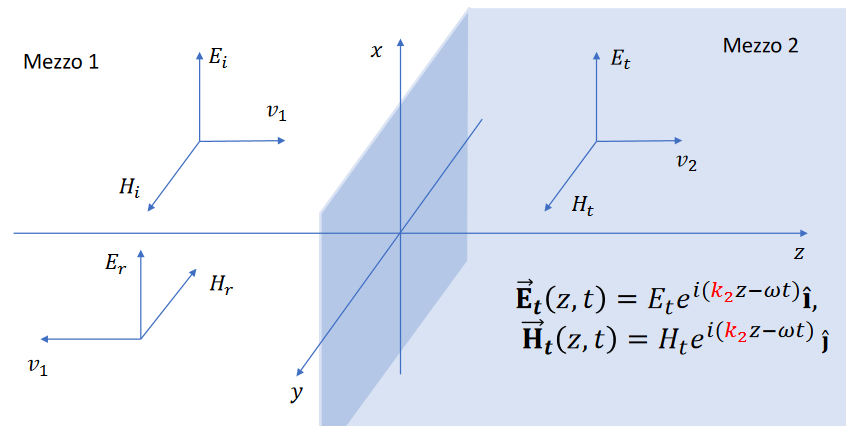
\includegraphics[width=0.5\textwidth]{screenshots/2024-05-07-11-22-20.png}
\end{figure}
Le onde incidenti sono \(\vec{E}_i(z,t)=E_i e^{i(k_1 z- \omega t)}\vec{\hat{i}}\) e \(\vec{H}_i(z,t)=H_i e^{i(k_1 z -\omega t)}\vec{\hat{j}}\). Si avranno onde riflesse:
\begin{align}
	\vec{E}_r(z,t) &= E_r e^{i(-k_1 z - \omega t)} \vec{\hat{i}} &
	\vec{H}_r(z,t) &= - H_r e^{i(-k_1 z - \omega t)} \vec{\hat{j}}
\end{align}
dove il segno di \(H_r\) è negativo per avere una terna destrorsa. Si hanno anche onde trasmesse:
\begin{align}
	\vec{E}_t(z,t)&=E_t e^{i(k_2 z -\omega t)} \vec{\hat{i}} &
	\vec{H}_t (z,t)&=H_t e^{i(k_2 z- \omega t)} \vec{\hat{j}}
\end{align}
Ricordo la relazione che sussiste fra \(\vec{H}\) e \(\vec{E}\) nelle onde elettromagnetiche:
\begin{gather}
	\vec{H} = \frac{\vec{k}}{\omega \mu } \cp \vec{E}\\
	\implies \vert \vec{H} \vert = \frac{\vert \vec{E} \vert }{Z}
\end{gather}
Le impedenze dipendono dall'impedenza del vuoto attraverso l'inverso dell'indice di rifrazione: \(Z_1 = \quotient{Z_0}{n_1}\) e \(Z_2 = \quotient{Z_0}{n_2} \).
Di conseguenza i moduli di \(\vec{H}\) ed \(\vec{E}\) possono essere collegati così:
\begin{align}
	H_i &= n_1 \frac{E_i}{Z_0} &
	H_r &= n_1 \frac{E_r}{Z_0} &
	H_t &= n_2 \frac{E_t}{Z_0}
\end{align}
Dobbiamo ora trovare le relazioni fra i campi elettrici.
\begin{figure}[H]
	\centering
	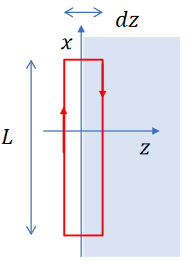
\includegraphics[width=0.3\textwidth]{screenshots/2024-05-07-11-32-18.png}
\end{figure}
Attraverso la curva rappresentata nella figura il flusso del campo magnetico tende a zero (l'area tende a zero), quindi la circuitazione del campo elettrico è nulla. Il contributo dei due lati piccoli tende a zero se i lati tendono a zero. Da questo segue che
\begin{equation}
	E_i + E_r = E_t
\end{equation}
Facciamo lo stesso ragionamento per il campo \(\vec{H}\). Non ci sono correnti concatenate e il flusso del campo elettrico attraverso la superficie tende a zero. Da questo segue che la circuitazione del campo \(\vec{H}\) è nulla, quindi
\begin{equation}
	H_i - H_r = H_t
\end{equation}
Il segno negativo davanti ad \(H_r\) deriva dal fatto che \(\vec{H}\) riflesso è opposto rispetto ad \(\vec{H}\) incidente.
Ho trovato un sistema di equazioni che mi permette di esplicitare i campi trasmessi e riflessi rispetto al campo incidente.
\begin{gather}
	\begin{cases}
		E_i +E_r = E_t\\
		n_1 \frac{E_i}{Z_0} - n_1 \frac{E_r}{Z_0} = n_2 \frac{E_t}{Z_0}
	\end{cases}
	\implies 
	\begin{cases}
		E_t = E_i + E_r\\
		n_1 E_i - n_1 E_r = n_2 E_i + n_2 E_r
	\end{cases}\\
	\implies 
	\begin{cases}
		E_t = \frac{2n_1}{n_1 + n_2} E_i\\
		E_r = \frac{n_1 - n_2}{n_1 + n_2} E_i
	\end{cases}
\end{gather}
Inserendo le impedenze possiamo trovare
\begin{formula}
	[Incidenza normale per le onde elettromagnetiche]
	\begin{align}
		&
		\begin{cases}
			E_t = \frac{2 Z_2}{Z_1 + Z_2} E_i\\
			E_r = \frac{Z_2 -Z_1}{Z_1 + Z_2} E_i
		\end{cases}
		&
		&
		\begin{cases}
			H_t = \frac{2 Z_1}{Z_1 + Z_2}H_i\\
			H_r = \frac{Z_2 - Z_1}{Z_1 + Z_2}
		\end{cases}
	\end{align}
	Queste formule sono state ricavate mantenendo fermo il verso del campo elettrico riflesso e ribaltando H (infatti al numeratore in \(H_r\) c'è \(Z_2 - Z_1\) e non \(Z_1 - Z_2\) come accadeva nelle onde meccaniche). Se avessimo tenuto fermo il verso del campo H per il campo riflesso avremmo ottenuto le stesse formule della corda.
\end{formula}

\begin{note}
	Questi risultati valgono anche per onde impulsive e per onde con polarizzazione diversa da quella lineare.
\end{note}

\subsection{Valutazione energetica}
Come nelle onde su corda, l'intensità dell'onda si conserva (è una forma di conservazione dell'energia).
\begin{figure}[H]
	\centering
	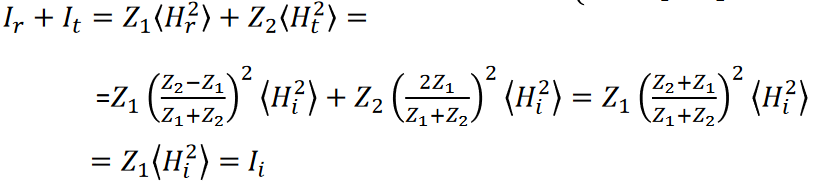
\includegraphics[width=0.5\textwidth]{screenshots/2024-05-07-11-55-08.png}
\end{figure}
Posso definire ancora i coefficienti di trasmissione e di riflessione:
\begin{definition}
	[Coefficienti di trasmissione e di riflessione]
	\begin{align}
		T &= \frac{4 Z_1 Z_2}{(Z_1 + Z_2)}^{2} &
		R &= \left( \frac{Z_2 - Z_1}{Z_1 + Z_2} \right)^{2}  
	\end{align}
	Per definizione \(R + T = 1\), \(I_t = T I_i\) e \(I_r = R I_i\).
\end{definition}

\subsection{Incidenza non normale}
Studiamo ora l'aspetto geometrico del passaggio fra due mezzi differenti, ossia come cambiano i versori che descrivono la direzione dell'onda.

\paragraph{Riflessione}
Si fa riferimento alla seguente figura e si sfrutta il principio di Huygens-Fresnel:
\begin{figure}[H]
	\centering
	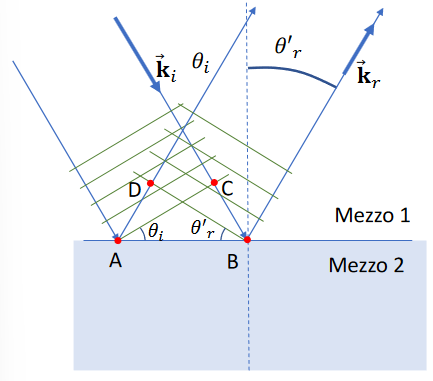
\includegraphics[width=0.4\textwidth]{screenshots/2024-05-07-12-17-10.png}
\end{figure}
Nel tempo in cui il punto C arriva in B, il punto A dello stesso fronte d'onda è arrivato in D (siamo sempre nel mezzo 1). I triangoli ABC e ABD sono entrambi retti per costruzione, perché sono dati dall'intersezione di un fronte d'onda con la retta di propagazione dell'onda. Inoltre hanno due lati uguali (AB in comune e AD=BC), quindi hanno anche gli stessi angoli. Segue che
\begin{equation}
	\theta^{\prime} _r = \theta _i
\end{equation}
Di conseguenza \(\vec{k}_i\), \(\vec{k}_r\) e la normale alla superficie stanno nello stesso piano, che è detto "piano d'incidenza".

\begin{note}
	Abbiamo parlato di riflessione nel caso di onde elettromagnetiche, ma il ragionamento si applica identico a tutti gli altri tipi di onde perché si basa esclusivamente sul principio di Huygens-Fresnel e caratteristiche generiche delle onde.
\end{note}

\paragraph{Rifrazione}
Consideriamo ora il caso della rifrazione, ossia la trasmissione con un angolo di incidenza diverso da zero rispetto alla normale.
\begin{figure}[H]
	\centering
	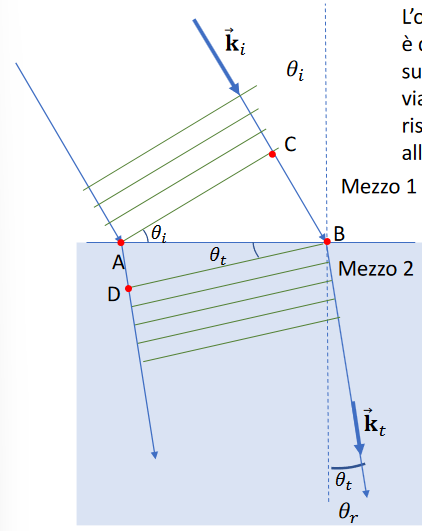
\includegraphics[width=0.4\textwidth]{screenshots/2024-05-07-12-26-14.png}
\end{figure}
Sia \(t_{CB} = \quotient{\overline{CB} }{v_1} \) il tempo che ci mette il punto C ad arrivare a B. Nello stesso tempo il punto A si muove in D: \(t_{AD} = \quotient{\overline{AD} }{v_2} = t_{CB} \). So anche che \(\overline{CB} = \overline{AB} \sin (\theta _i)\) e \(\overline{AD} = \overline{AB} \sin (\theta _t)\), quindi trovo
\begin{equation}
	\frac{\overline{AD} }{v_2} = \frac{\overline{CB} }{v_1}
	\implies \frac{\overline{AB} \sin (\theta _t)}{v_2} = \frac{\overline{AB} \sin (\theta _i)}{v_1}
	\implies \frac{n_2 \sin (\theta _t)}{c} = \frac{n_1 \sin (\theta _i)}{c}
\end{equation}
Così otteniamo la legge di Snell per la rifrazione:
\begin{formula}
	[Legge di Snell]
	\begin{equation}
		n_1 \sin (\theta _i) = n_2 \sin (\theta _r)
	\end{equation}
\end{formula}
Passando da un mezzo con indice di rifrazione basso ad uno con indice di rifrazione alto (\(n_1 < n_2\)) la direzione dell'onda si avvicina alla normale, quindi \(\theta _r < \theta _i\). Viceversa, passando da un mezzo con indice di rifrazione alto ad uno con indice di rifrazione basso (\(n_1 > n_2\)) la direzione dell'onda si allontana dalla normale, ossia \(\theta _r > \theta _i\) (non sempre è possibile!). Essendo \(\sin (\theta _r) = \frac{n_1}{n_2} \sin (\theta _i)\), se \(\sin (\theta _i)> \frac{n_2}{n_1}\) non esiste alcun \(\theta _r\) che soddisfi l'equazione. Sono nel caso della \emph{riflessione totale}. Non avviene la rifrazione, ma avviene solo la riflessione. Succede ad esempio in piscina buttandosi sott'acqua e guardando verso l'alto.

\paragraph{Applicazione: fibra ottica}
Le fibre ottiche sfruttano il fenomeno della riflessione totale. All'interno c'è il core con indice \(n\), subito fuori c'è il cladding con indice \(n_c\) e a protezione c'è una guaina protettiva non trasparente.
\begin{figure}[H]
	\centering
	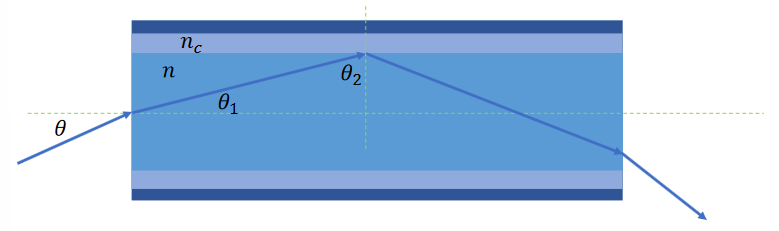
\includegraphics[width=0.5\textwidth]{screenshots/2024-05-07-12-43-10.png}
\end{figure}
Si definisce l'apertura numerica della fibra \(NA=\sin (\theta_{max} = \sqrt{n^{2} -n_c ^{2} } )\) dove \(\theta_{max} \) è il massimo angolo di incidenza per cui si ha riflessione totale all'incidenza sul cladding. Per angoli più piccoli (rispetto alla normale) si ha anche rifrazione, ma è possibile evitare che succeda. Questo mi permette di curvare la luce!

\paragraph{Applicazione: prisma}
Su una lastra di vetro a facce parallele un raggio che entra all'angolo \(\theta \) esce con lo stesso angolo indipendentemente dall'indice di rifrazione del vetro (si vede applicando la legge di Snell). Nel prisma le facce non sono parallele, ne consegue che l'angolo di uscita è una funzione dell'indice di rifrazione e dell'angolo incidente: \(\theta_f = f(n, \theta _i)\). Poiché \(n =n(\lambda )\), ne consegue che un fascio di luce bianca si separa in uno spettro di colori. È lo stesso fenomeno fisico che accade nelle gocce d'acqua e che permette la formazione dell'arcobaleno.

\paragraph{Principio di Fermat}
Il principio di Fermat generalizza la legge di Snell e la formalizza in una sorta di principio di minima azione. Tra tutti i possibili cammini che un raggio di luce può percorrere per andare da un punto a un altro, esso segue il cammino che richiede il tempo più breve.
\begin{figure}[H]
	\centering
	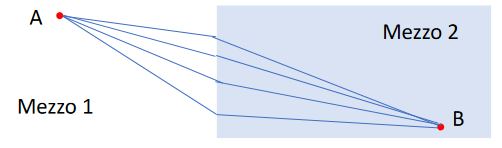
\includegraphics[width=0.35\textwidth]{screenshots/2024-05-07-12-54-12.png}
\end{figure}
Il tempo necessario ad andare dal punto A al punto B è
\begin{equation}
	T = \int \frac{\mathrm{d} l}{v} = \frac{1}{c} \int n \mathrm{d} l
\end{equation}
Minimizzare il tempo significa minimizzare il percorso ottico: \(L_{ott}  \int n \mathrm{d} l\).

\begin{exercise}
	Per casa, prova a ottenere la legge di Snell a partire dal principio di Fermat.
\end{exercise}